\documentclass[11pt]{article}

\usepackage[a4paper,margin=1in]{geometry}
\usepackage{amsmath,amssymb,amsthm,mathtools}
\usepackage{enumitem}
\usepackage{hyperref}
\usepackage[x11names,dvipsnames,svgnames]{xcolor}
\usepackage{listings}
\usepackage[T1]{fontenc}
\usepackage[utf8]{inputenc}
\usepackage{microtype}

\definecolor{codegreen}{rgb}{0,0.6,0}
\definecolor{codegray}{rgb}{0.5,0.5,0.5}
\definecolor{codepurple}{rgb}{0.58,0,0.82}
\definecolor{backcolour}{rgb}{0.98,0.98,0.98}

\lstdefinestyle{pythonstyle}{
  language=Python,
  backgroundcolor=\color{backcolour},
  commentstyle=\color{codegreen},
  keywordstyle=\color{magenta},
  numberstyle=\tiny\color{codegray},
  stringstyle=\color{codepurple},
  basicstyle=\ttfamily\small,
  columns=fullflexible,
  showstringspaces=false,
  keepspaces=true,
  frame=single,
  framerule=0.2pt,
  breaklines=true,
  numbers=left,
  numbersep=5pt,
}

\lstset{style=pythonstyle}

\newtheorem{definition}{Definition}
\newtheorem{proposition}{Proposition}
\newtheorem{remark}{Remark}
\newtheorem{example}{Example}

\newcommand{\G}{\mathcal{G}}
\newcommand{\F}{\mathcal{F}}
\newcommand{\Dom}{\mathrm{Dom}}
\newcommand{\Domb}{\mathrm{Dom}_b}
\DeclareMathOperator*{\argmax}{arg\,max}

\title{Partial Functions and Preference for ARC:\\
Domains, Interpolation, and Adaptation (Research Note)}
\author{Cristiano Calcagno}
\date{2025-10-31}

\begin{document}
\maketitle

\begin{abstract}
We formalize Abstraction and Reasoning Corpus (ARC) tasks using partial functions over grids and a numeric preference function on programs. The central concept is the \emph{behavioural domain} that encodes the programmer's intended coverage. We give a short calculus for behavioural definedness under boolean connectives, characterize interpolation, generalisation, and adaptation to novelty, and work through a representative example where generalisation succeeds precisely by extending the behavioural domain to include a previously unhandled color.
\end{abstract}

\section{Model}

\begin{definition}[Objects]
Let $\G$ be the set of grids. Candidate programs are partial functions $f:\G\rightharpoonup \G$; write $\Domb(f)\subseteq \G$ for the (behavioural) domain of $f$, i.e.\ the set of inputs on which $f$ \emph{specifies} behaviour. Let $\F$ denote a chosen hypothesis class of such programs.
\end{definition}

\begin{definition}[Preference]
A numeric scoring function $P:\F\to\mathbb{R}$ induces a strict preference: $f_1$ is preferred to $f_2$ iff $P(f_1)>P(f_2)$.
\end{definition}

\begin{definition}[ARC puzzles]
An ARC puzzle (instance) consists of training pairs $\{(i_k,o_k)\}_{k=1}^n\subseteq \G\times\G$ and a test input $i\in\G$.
\end{definition}

\begin{definition}[Interpolants]
For training pairs $\{(i_k,o_k)\}_{k=1}^n$, a program $f$ \emph{interpolates} the training set if for all $k$, $i_k\in\Domb(f)$ and $f(i_k)=o_k$. Let $\mathcal{I}=\{f\in\F\mid f \text{ interpolates } \{(i_k,o_k)\}_{k=1}^n\}$ denote the set of all interpolants.
\end{definition}

\begin{definition}[Tentative solution, solution, ambiguity/void]
A \emph{tentative solution} is any interpolant $f\in\mathcal{I}$ such that $i\in\Domb(f)$. Let
\[
\mathcal{S} \;=\; \bigl\{ f\in\mathcal{I} \,\big|\, i\in\Domb(f)\bigr\}.
\]
The \emph{intended solution} is any $f^\star\in \argmax_{f\in\mathcal{S}} P(f)$ (i.e., the element of~$\mathcal{S}$ that maximizes~$P$). The instance is \emph{void} if $\mathcal{S}=\varnothing$ and \emph{ambiguous} if $|\argmax_{f\in\mathcal{S}} P(f)|>1$.
\end{definition}

\begin{definition}[Generalisation and adaptation to novelty]
\emph{Generalisation} is moving between interpolants $f,g\in\mathcal{I}$ with $P(g)>P(f)$. The top-scoring interpolant $f^\dagger\in\argmax_{f\in\mathcal{I}}P(f)$ (the interpolant maximizing~$P$) may fail to cover the test input ($i\notin\Domb(f^\dagger)$). \emph{Adaptation to novelty} selects a tentative solution $g^\star\in\argmax_{f\in\mathcal{S}}P(f)$; since $\mathcal{S}\subseteq\mathcal{I}$, necessarily $P(g^\star)\le P(f^\dagger)$.
\end{definition}

This formulation clarifies the tension in ARC: generalisation seeks higher-scoring interpolants (simpler, more elegant programs), while adaptation prioritizes coverage of the test input. When the test introduces novel features absent in training (e.g., a new color), the top interpolant $f^\dagger$ may exclude that case from $\Domb$, forcing a trade-off: accept a lower-preference tentative solution $g^\star$ that extends the behavioural domain, or stick with $f^\dagger$ and risk failure.

\section{Behavioural domain}

We focus on the \textbf{behavioural domain} $\Domb(e)$: the inputs on which the specification intends to define behaviour (coverage). We assume standard short-circuit evaluation for expressions; runtime definedness is incidental here and not our emphasis.

\paragraph{Definedness calculus (examples).}
For boolean expressions $E,F$ and comparisons $x{=}c$,
\begin{align}
\Domb(\lnot E) &= \Domb(E), \label{eq:not}\\
\Domb((x{=}c \land E) \lor F) &= (x{=}c \land \Domb(E)) \lor \Domb(F). \label{eq:conjdisj}
\end{align}
For a DSL primitive $g(\cdot)$, we assume a given predicate $\Domb(g)$.

\section{Worked example}

We illustrate the role of the behavioural domain using ARC-AGI-2 task dfadab01. The puzzle is available at \url{https://arcprize.org/play?task=dfadab01}; the full solver analysis at \url{https://gist.github.com/cristianoc/e86779cee94658567ecba429133d6667}.

Consider the following (corrected) DSL function:
\begin{lstlisting}
def valid_anchor(grid: Grid, anchor: Anchor) -> bool:
    row, col, color = anchor
    return not (
        (color == 2 and guard_nw_eq(grid, (row, col), 4))
        or (color == 5 and guard_nw_eq(grid, (row, col), 6))
    )
\end{lstlisting}
% Inline the guard primitives directly (no G4/G6 abbreviations).

\begin{example}[Behavioural domain]
If the intended specification handles only colors $2$ (red) and $5$ (gray), the behavioural domain must be:
\[
\begin{aligned}
\Domb(\texttt{valid\_anchor})
&= (color{=}2 \land \Domb(\texttt{guard\_nw\_eq}(grid,(row,col),4))) \\
&\quad \lor (color{=}5 \land \Domb(\texttt{guard\_nw\_eq}(grid,(row,col),6))).
\end{aligned}
\]
This captures the explicit color-specific guards: only when color is $2$ do we check the guard for color $4$, and only when color is $5$ do we check the guard for color $6$. Any other color falls outside the intended behavioural domain.
\end{example}

\begin{remark}[Novelty at test time]
If the test input has \texttt{color}$=8$ (sky blue), then the expression \emph{computationally} evaluates (no guard is forced), but $i\notin\Domb(\texttt{valid\_anchor})$ by the behavioural domain example above. Generalisation must therefore extend the behavioural domain (e.g.\ add a new branch or a principled fallback) so that $8$ becomes covered.
\end{remark}

\begin{figure}[ht]
\centering
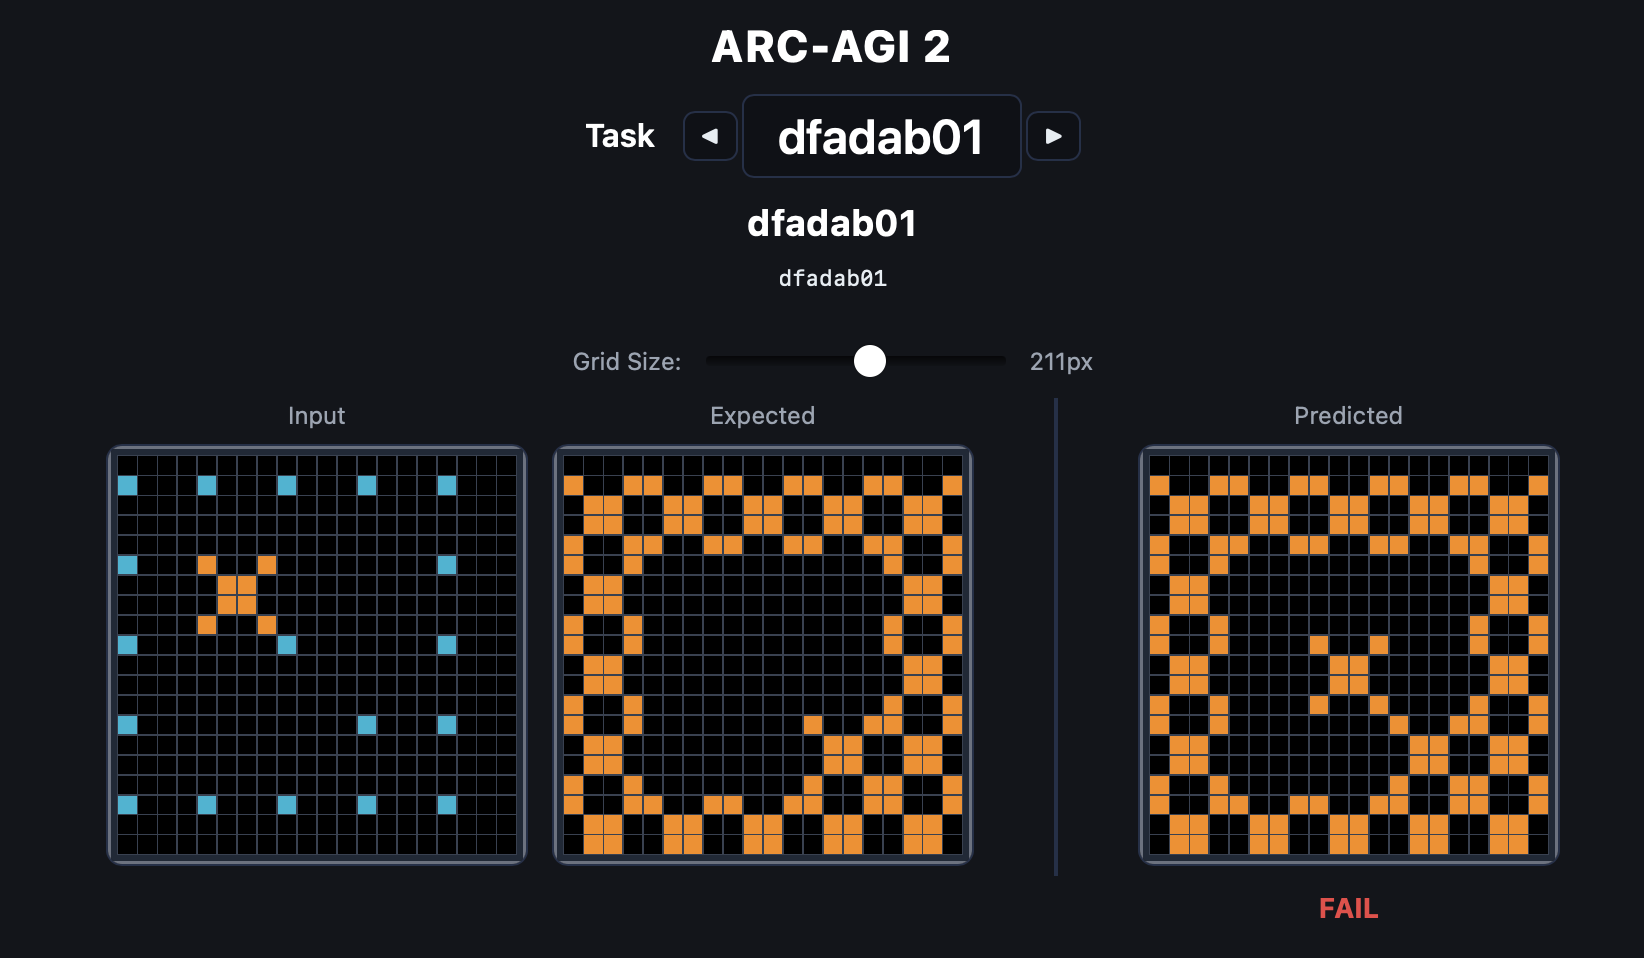
\includegraphics[width=0.9\textwidth]{images/solver_comparison.png}
\caption{Before/after comparison showing domain extension failure and recovery: the initial solver explicitly handles only red ($2$) and gray ($5$). When sky blue ($8$) appears in the test input (corresponding to an \texttt{X}-pattern motif with orange ($7$) borders), the solver incorrectly stamps the motif because $8 \notin \Domb(\texttt{valid\_anchor})$. The simplified version introduces \texttt{guard\_color} (deriving the guard color $7$ from the motif's top-left cell) to uniformly treat all motifs, extending $\Domb$ to include color $8$ and preventing spurious stamping.}
\label{fig:comparison}
\end{figure}

\section{Practical Implications}

The model suggests a concrete operating procedure and design tips:
\begin{itemize}[leftmargin=1.5em]
\item \textbf{Selection rule.} Among interpolants, pick the tentative solutions that cover the test ($\mathcal{S}$) and choose the $P$-maximizer; if $\mathcal{S}=\varnothing$ the instance is \emph{void}, and if multiple maximizers remain it is \emph{ambiguous}.
\item \textbf{Novelty handling.} If the top-scoring interpolant $f^\dagger$ does not cover the test ($i\notin \Domb(f^\dagger)$), extend the behavioural domain with the minimal, principled change that includes $i$, accepting a possible decrease in~$P$.
\item \textbf{Make coverage explicit.} Encode intended coverage via guard-style case-splits with no default \texttt{else}; this makes $\Domb$ visible and simplifies reasoning about what inputs are intentionally handled.
\item \textbf{Debugging checklist.} On failures, first distinguish evaluation errors from coverage gaps: compute or approximate $\Domb(e)$ for the failing expression and check whether the test input lies outside it.
\end{itemize}

\section{Summary}

Modeling ARC programs as partial functions with a numeric score yields a compact account of interpolation, generalisation, and adaptation. The \emph{behavioural domain} is essential: many failures are not evaluation errors but \emph{coverage} gaps. In the example, the initial solver fails on the test because color $8$ is outside $\Domb$; the generalised solution succeeds precisely by extending $\Domb$ to include that case.

\end{document}
